\vspace{.5cm}
\begin{table}[h]
    \centering
    \begin{tabular}{c|c}
        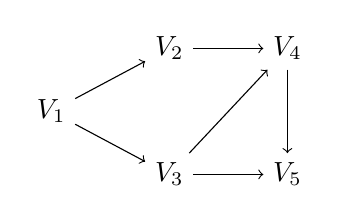
\begin{tikzpicture}
            \node (1) at (0,0) {$V_1$};
            \node (2) at (1.5,.8) {$V_2$};
            \node (3) at (1.5,-.8) {$V_3$};
            \node (4) at (3,.8) {$V_4$};
            \node (5) at (3,-.8) {$V_5$};
            \draw[->]  (1) edge (2);
            \draw[->]  (1) edge (3);
            \draw[->]  (2) edge (4);
            \draw[->]  (3) edge (5);
            \draw[->]  (3) edge (4);
            \draw[->]  (4) edge (5);
        \end{tikzpicture}
        \hspace{.5cm}
        &
        \hspace{.5cm}
        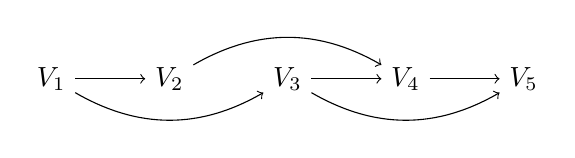
\begin{tikzpicture}
            \node (1) at (0,0) {$V_1$};
            \node (2) at (1.5,0) {$V_2$};
            \node (3) at (3,0) {$V_3$};
            \node (4) at (4.5,0) {$V_4$};
            \node (5) at (6,0) {$V_5$};
            \draw[->]  (1) edge (2);
            \draw[->,bend right]  (1) edge (3);
            \draw[->,bend right]  (3) edge (5);
            \draw[->,bend left]  (2) edge (4);
            \draw[->]  (3) edge (4);
            \draw[->]  (4) edge (5);
        \end{tikzpicture}
    \end{tabular}
    \caption{DAG and its topological ordering.}
    \label{tab:topological}
\end{table}
\vspace{.5cm}